% Created by tikzDevice version 0.12.3.1 on 2022-09-01 15:55:23
% !TEX encoding = UTF-8 Unicode
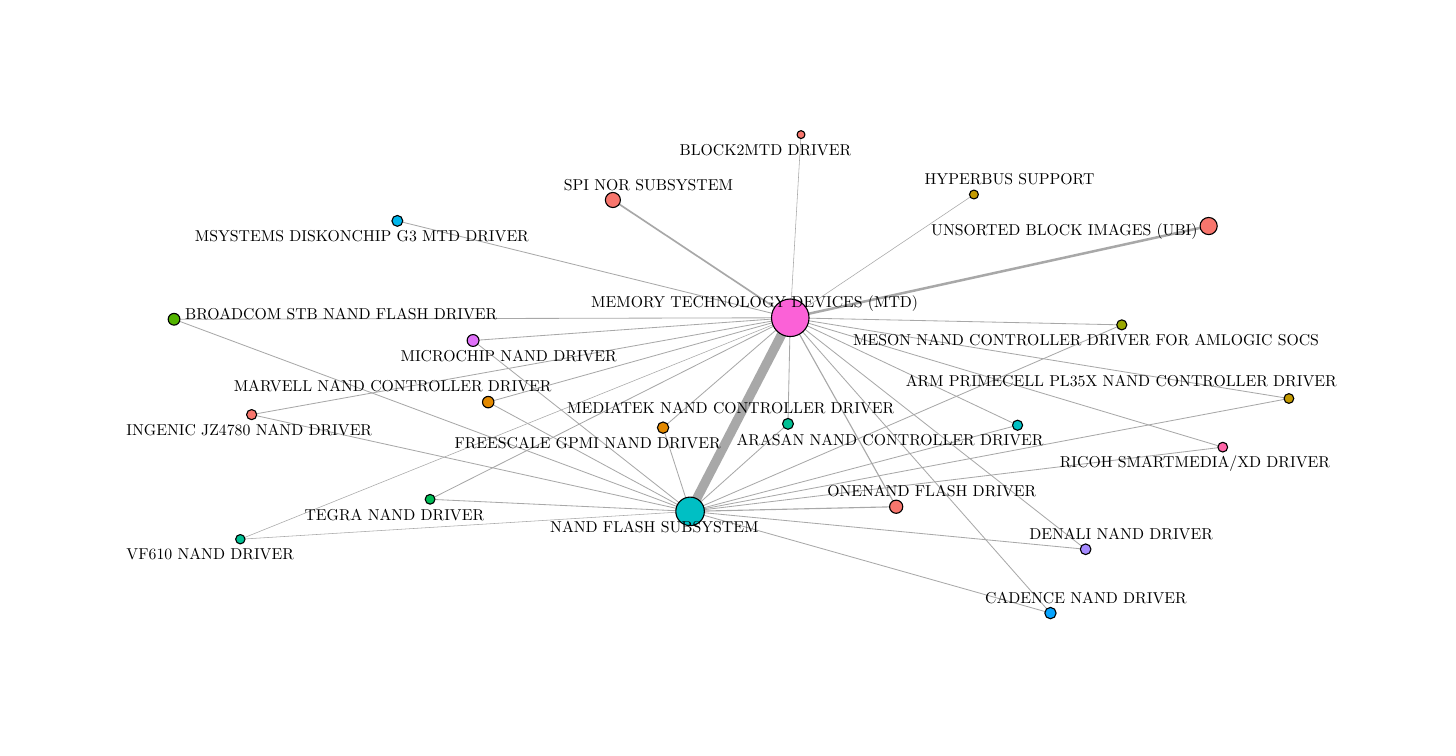
\begin{tikzpicture}[x=1pt,y=1pt]
\definecolor{fillColor}{RGB}{255,255,255}
\path[use as bounding box,fill=fillColor,fill opacity=0.00] (0,0) rectangle (505.89,252.94);
\begin{scope}
\path[clip] (  0.00,  0.00) rectangle (505.89,252.94);
\definecolor{fillColor}{RGB}{255,255,255}

\path[fill=fillColor] (  0.00,  0.00) rectangle (505.89,252.94);
\end{scope}
\begin{scope}
\path[clip] ( 32.75, 32.75) rectangle (475.89,222.94);
\definecolor{drawColor}{gray}{0.66}

\path[draw=drawColor,line width= 0.3pt,line join=round] (357.69,109.28) -- (275.56,148.11);

\path[draw=drawColor,line width= 0.3pt,line join=round] (357.69,109.28) -- (239.36, 78.15);

\path[draw=drawColor,line width= 0.3pt,line join=round] (455.75,118.94) -- (275.56,148.11);

\path[draw=drawColor,line width= 0.3pt,line join=round] (455.75,118.94) -- (239.36, 78.15);

\path[draw=drawColor,line width= 0.2pt,line join=round] (279.44,214.30) -- (275.56,148.11);

\path[draw=drawColor,line width= 0.3pt,line join=round] ( 52.89,147.57) -- (275.56,148.11);

\path[draw=drawColor,line width= 0.3pt,line join=round] ( 52.89,147.57) -- (239.36, 78.15);

\path[draw=drawColor,line width= 0.3pt,line join=round] (369.58, 41.40) -- (275.56,148.11);

\path[draw=drawColor,line width= 0.3pt,line join=round] (369.58, 41.40) -- (239.36, 78.15);

\path[draw=drawColor,line width= 0.3pt,line join=round] (382.29, 64.46) -- (275.56,148.11);

\path[draw=drawColor,line width= 0.3pt,line join=round] (382.29, 64.46) -- (239.36, 78.15);

\path[draw=drawColor,line width= 0.3pt,line join=round] (229.60,108.41) -- (275.56,148.11);

\path[draw=drawColor,line width= 0.3pt,line join=round] (229.60,108.41) -- (239.36, 78.15);

\path[draw=drawColor,line width= 0.2pt,line join=round] (341.93,192.65) -- (275.56,148.11);

\path[draw=drawColor,line width= 0.3pt,line join=round] ( 80.93,113.11) -- (275.56,148.11);

\path[draw=drawColor,line width= 0.3pt,line join=round] ( 80.93,113.11) -- (239.36, 78.15);

\path[draw=drawColor,line width= 0.3pt,line join=round] (166.42,117.63) -- (275.56,148.11);

\path[draw=drawColor,line width= 0.3pt,line join=round] (166.42,117.63) -- (239.36, 78.15);

\path[draw=drawColor,line width= 0.3pt,line join=round] (274.73,109.78) -- (275.56,148.11);

\path[draw=drawColor,line width= 0.3pt,line join=round] (274.73,109.78) -- (239.36, 78.15);

\path[draw=drawColor,line width= 0.3pt,line join=round] (275.56,148.11) -- (395.35,145.55);

\path[draw=drawColor,line width= 0.3pt,line join=round] (275.56,148.11) -- (160.94,139.90);

\path[draw=drawColor,line width= 0.3pt,line join=round] (275.56,148.11) -- (133.58,183.12);

\path[draw=drawColor,line width= 3.4pt,line join=round] (275.56,148.11) -- (239.36, 78.15);

\path[draw=drawColor,line width= 0.4pt,line join=round] (275.56,148.11) -- (313.83, 79.83);

\path[draw=drawColor,line width= 0.3pt,line join=round] (275.56,148.11) -- (431.85,101.36);

\path[draw=drawColor,line width= 0.6pt,line join=round] (275.56,148.11) -- (211.47,190.67);

\path[draw=drawColor,line width= 0.3pt,line join=round] (275.56,148.11) -- (145.41, 82.52);

\path[draw=drawColor,line width= 0.9pt,line join=round] (275.56,148.11) -- (426.74,181.26);

\path[draw=drawColor,line width= 0.2pt,line join=round] (275.56,148.11) -- ( 76.84, 68.09);

\path[draw=drawColor,line width= 0.3pt,line join=round] (395.35,145.55) -- (239.36, 78.15);

\path[draw=drawColor,line width= 0.3pt,line join=round] (160.94,139.90) -- (239.36, 78.15);

\path[draw=drawColor,line width= 0.4pt,line join=round] (239.36, 78.15) -- (313.83, 79.83);

\path[draw=drawColor,line width= 0.3pt,line join=round] (239.36, 78.15) -- (431.85,101.36);

\path[draw=drawColor,line width= 0.3pt,line join=round] (239.36, 78.15) -- (145.41, 82.52);

\path[draw=drawColor,line width= 0.2pt,line join=round] (239.36, 78.15) -- ( 76.84, 68.09);
\definecolor{drawColor}{RGB}{0,0,0}
\definecolor{fillColor}{RGB}{0,191,196}

\path[draw=drawColor,line width= 0.4pt,line join=round,line cap=round,fill=fillColor] (357.69,109.28) circle (  1.83);
\definecolor{fillColor}{RGB}{196,154,0}

\path[draw=drawColor,line width= 0.4pt,line join=round,line cap=round,fill=fillColor] (455.75,118.94) circle (  1.76);
\definecolor{fillColor}{RGB}{248,118,109}

\path[draw=drawColor,line width= 0.4pt,line join=round,line cap=round,fill=fillColor] (279.44,214.30) circle (  1.43);
\definecolor{fillColor}{RGB}{83,180,0}

\path[draw=drawColor,line width= 0.4pt,line join=round,line cap=round,fill=fillColor] ( 52.89,147.57) circle (  2.12);
\definecolor{fillColor}{RGB}{6,164,255}

\path[draw=drawColor,line width= 0.4pt,line join=round,line cap=round,fill=fillColor] (369.58, 41.40) circle (  2.05);
\definecolor{fillColor}{RGB}{165,138,255}

\path[draw=drawColor,line width= 0.4pt,line join=round,line cap=round,fill=fillColor] (382.29, 64.46) circle (  1.93);
\definecolor{fillColor}{RGB}{227,137,0}

\path[draw=drawColor,line width= 0.4pt,line join=round,line cap=round,fill=fillColor] (229.60,108.41) circle (  2.05);
\definecolor{fillColor}{RGB}{196,154,0}

\path[draw=drawColor,line width= 0.4pt,line join=round,line cap=round,fill=fillColor] (341.93,192.65) circle (  1.61);
\definecolor{fillColor}{RGB}{248,118,109}

\path[draw=drawColor,line width= 0.4pt,line join=round,line cap=round,fill=fillColor] ( 80.93,113.11) circle (  1.83);
\definecolor{fillColor}{RGB}{227,137,0}

\path[draw=drawColor,line width= 0.4pt,line join=round,line cap=round,fill=fillColor] (166.42,117.63) circle (  2.07);
\definecolor{fillColor}{RGB}{0,192,148}

\path[draw=drawColor,line width= 0.4pt,line join=round,line cap=round,fill=fillColor] (274.73,109.78) circle (  1.97);
\definecolor{fillColor}{RGB}{251,97,215}

\path[draw=drawColor,line width= 0.4pt,line join=round,line cap=round,fill=fillColor] (275.56,148.11) circle (  6.78);
\definecolor{fillColor}{RGB}{153,168,0}

\path[draw=drawColor,line width= 0.4pt,line join=round,line cap=round,fill=fillColor] (395.35,145.55) circle (  1.82);
\definecolor{fillColor}{RGB}{223,112,248}

\path[draw=drawColor,line width= 0.4pt,line join=round,line cap=round,fill=fillColor] (160.94,139.90) circle (  2.14);
\definecolor{fillColor}{RGB}{0,182,235}

\path[draw=drawColor,line width= 0.4pt,line join=round,line cap=round,fill=fillColor] (133.58,183.12) circle (  1.96);
\definecolor{fillColor}{RGB}{0,191,196}

\path[draw=drawColor,line width= 0.4pt,line join=round,line cap=round,fill=fillColor] (239.36, 78.15) circle (  5.16);
\definecolor{fillColor}{RGB}{248,118,109}

\path[draw=drawColor,line width= 0.4pt,line join=round,line cap=round,fill=fillColor] (313.83, 79.83) circle (  2.38);
\definecolor{fillColor}{RGB}{255,102,168}

\path[draw=drawColor,line width= 0.4pt,line join=round,line cap=round,fill=fillColor] (431.85,101.36) circle (  1.76);
\definecolor{fillColor}{RGB}{248,118,109}

\path[draw=drawColor,line width= 0.4pt,line join=round,line cap=round,fill=fillColor] (211.47,190.67) circle (  2.72);
\definecolor{fillColor}{RGB}{0,188,86}

\path[draw=drawColor,line width= 0.4pt,line join=round,line cap=round,fill=fillColor] (145.41, 82.52) circle (  1.77);
\definecolor{fillColor}{RGB}{248,118,109}

\path[draw=drawColor,line width= 0.4pt,line join=round,line cap=round,fill=fillColor] (426.74,181.26) circle (  3.10);
\definecolor{fillColor}{RGB}{0,192,148}

\path[draw=drawColor,line width= 0.4pt,line join=round,line cap=round,fill=fillColor] ( 76.84, 68.09) circle (  1.69);

\node[text=drawColor,anchor=base,inner sep=0pt, outer sep=0pt, scale=  0.57] at (311.64,101.80) {ARASAN NAND CONTROLLER DRIVER};

\node[text=drawColor,anchor=base,inner sep=0pt, outer sep=0pt, scale=  0.57] at (395.16,123.26) {ARM PRIMECELL PL35X NAND CONTROLLER DRIVER};

\node[text=drawColor,anchor=base,inner sep=0pt, outer sep=0pt, scale=  0.57] at (266.56,206.83) {BLOCK2MTD DRIVER};

\node[text=drawColor,anchor=base,inner sep=0pt, outer sep=0pt, scale=  0.57] at (113.29,147.59) {BROADCOM STB NAND FLASH DRIVER};

\node[text=drawColor,anchor=base,inner sep=0pt, outer sep=0pt, scale=  0.57] at (382.39, 44.95) {CADENCE NAND DRIVER};

\node[text=drawColor,anchor=base,inner sep=0pt, outer sep=0pt, scale=  0.57] at (395.11, 68.01) {DENALI NAND DRIVER};

\node[text=drawColor,anchor=base,inner sep=0pt, outer sep=0pt, scale=  0.57] at (202.32,100.92) {FREESCALE GPMI NAND DRIVER};

\node[text=drawColor,anchor=base,inner sep=0pt, outer sep=0pt, scale=  0.57] at (354.79,196.21) {HYPERBUS SUPPORT};

\node[text=drawColor,anchor=base,inner sep=0pt, outer sep=0pt, scale=  0.57] at ( 80.07,105.60) {INGENIC JZ4780 NAND DRIVER};

\node[text=drawColor,anchor=base,inner sep=0pt, outer sep=0pt, scale=  0.57] at (131.87,121.63) {MARVELL NAND CONTROLLER DRIVER};

\node[text=drawColor,anchor=base,inner sep=0pt, outer sep=0pt, scale=  0.57] at (254.02,113.36) {MEDIATEK NAND CONTROLLER DRIVER};

\node[text=drawColor,anchor=base,inner sep=0pt, outer sep=0pt, scale=  0.57] at (262.68,151.69) {MEMORY TECHNOLOGY DEVICES (MTD)};

\node[text=drawColor,anchor=base,inner sep=0pt, outer sep=0pt, scale=  0.57] at (382.43,138.06) {MESON NAND CONTROLLER DRIVER FOR AMLOGIC SOCS};

\node[text=drawColor,anchor=base,inner sep=0pt, outer sep=0pt, scale=  0.57] at (173.81,132.43) {MICROCHIP NAND DRIVER};

\node[text=drawColor,anchor=base,inner sep=0pt, outer sep=0pt, scale=  0.57] at (120.76,175.64) {MSYSTEMS DISKONCHIP G3 MTD DRIVER};

\node[text=drawColor,anchor=base,inner sep=0pt, outer sep=0pt, scale=  0.57] at (226.45, 70.64) {NAND FLASH SUBSYSTEM};

\node[text=drawColor,anchor=base,inner sep=0pt, outer sep=0pt, scale=  0.57] at (326.69, 83.38) {ONENAND FLASH DRIVER};

\node[text=drawColor,anchor=base,inner sep=0pt, outer sep=0pt, scale=  0.57] at (421.77, 93.89) {RICOH SMARTMEDIA/XD DRIVER};

\node[text=drawColor,anchor=base,inner sep=0pt, outer sep=0pt, scale=  0.57] at (224.30,194.23) {SPI NOR SUBSYSTEM};

\node[text=drawColor,anchor=base,inner sep=0pt, outer sep=0pt, scale=  0.57] at (132.50, 75.03) {TEGRA NAND DRIVER};

\node[text=drawColor,anchor=base,inner sep=0pt, outer sep=0pt, scale=  0.57] at (374.62,177.86) {UNSORTED BLOCK IMAGES (UBI)};

\node[text=drawColor,anchor=base,inner sep=0pt, outer sep=0pt, scale=  0.57] at ( 65.95, 60.59) {VF610 NAND DRIVER};
\end{scope}
\end{tikzpicture}
